% Chapter 1

\chapter{Numerical Simulation of Solidification Process} % Main chapter title

\label{Chapter3} % For referencing the chapter elsewhere, use \ref{Chapter1} 
\section{OpenFOAM. General Aspects}
OpenFOAM is a free open-source software written in C++ and mainly conceived to perform computational fluid dynamics (CFD) simulations based on a finite volume discretization. 
In this first section, a brief introduction on the structure and functioning of the OpenFOAM software is given.
In the folder structure tree shown in Fig. \ref{fig:structureOF}, it is shown a typical case setup for a phase change problem using \textit{icoReactingMultiphaseFoam} solver.
\clearpage
\begin{figure}[h!]
	\centering
	\scalebox{0.75}{
	\begin{forest}
		for tree={
			font=\ttfamily,
			grow'=0,
			child anchor=west,
			parent anchor=south,
			anchor=west,
			calign=first,
			edge path={
				\noexpand\path [draw, \forestoption{edge}]
				(!u.south west) +(7.5pt,0) |- node[fill,inner sep=1.25pt] {} (.child anchor)\forestoption{edge label};
			},
			before typesetting nodes={
				if n=1
				{insert before={[,phantom]}}
				{}
			},
			fit=band,
			before computing xy={l=15pt},
		}
		[phaseChangeCase
		[0*
		[alpha.liquid]
		[alpha.solid]
		[p]
		[$p_{rgh}$]
		[T]
		[U]
		]
		[constant*
		[g]
		[phaseProperties]
		[thermophysicalProperties.liquid]
		[thermophysicalProperties.solid]
		[turbulenceProperties]
		[polyMesh]
		]
		[system*
		[blockMeshDict]
		[controlDict]
		[decomposeParDict]
		[fvSchemes]
		[fvSolution]
		]
		]
	\end{forest}}
	\label{fig:structureOF}
	\caption{General structure of an OpenFOAM case.}
\end{figure}

\subsection{Boundary Conditions Directory}
The "0" directory gathers all the boundary conditions at time zero and the initial conditions to set up the case. As the simulation starts running, the information of these fields is saved in folders at every timestep.
\subsection{Constant Properties Directory}
The "constant" directory contains all the information typically regarding the physical properties which are kept constant through the simulation. Moreover, once the dictionary \textit{blockMeshDict} is run, OpenFOAM creates a folder called \textit{polyMesh} containing all the information relevant to the mesh (points, faces,...) 
\subsection{System Directory}
This folder contains the files required by the control of the solver and the solution itself. The most common files are:
\begin{itemize}
	\item \textbf{blockMeshDict:} in this file the parameters required to build up the computational domain, the mesh and the boundaries are found. The command \textbf{blockMesh} executes this dictionary creating the \textit{polyMesh} folder commented above.
	\item \textbf{controlDict:} Time parameters associated to the computation are set in this file. 
	\item \textbf{decomposeParDict:} In the realization of this thesis, the help of parallel computing is required. Thus, in this file, parameters regarding the decomposition of the mesh are configured. It is executed by means of the \textbf{decomposePar} appliation implicit in OF. The mesh is afterwards reconstructed by using \textbf{reconstructPar} 
	\item \textbf{fvSchemes:} Schemes selected for the discretization of the derivative terms are defined. Among others, time schemes, gradient schemes, laplacian schemes, divergent schemes, interpolation schemes can be declared here.
	\item \textbf{fvSolution:} contains sub-dictionaries used to control the solvers and the solution algorithms. It also allows the definition of the fields resolution.
\end{itemize}


\section{Solidification process. Methodology}
A convection solver is used to represent the flow behavior generated by the density difference due to existing temperature gradients whithin the volume of control. A polynomic water density is implemented in the native OpenFOAM solver and compared with the standard Boussinesq approximation. The current model is validated against numerical results form the literature. The solution of this convection solver is later used as a boundary condition, before solidification phenomena plays a role.

\newpage
\section{OpenFOAM: BuoyantBoussinesqPimpleFOAM. Natural Convection solver}

In a natural convection environment, the motion of the fluid is mainly driven by the density difference within the fluid volume of control. At its turn, the differences in the density, responsible for buoyancy forces, are generated by the existing temperature gradients. Within a physical context, the fluid near a hot heat source gets warmed up and, as a result, it becomes less dense moving up inside a domain. Consequently, the fluid in contact of the cold heat source is pushed from its zone to replace the hot fluid location. At this point, the cycle starts again repeating the phyisical phenomena.
\subsection{Control Loop}
The \textit{buoyantBoussinesqPimpleFoam} is a solver used to solve non-steady buoyancy-driven fluids by using the Boussinesq approximation as a coupling between density and temperature fields. It considers the fluid as incompressible and uses the PIMPLE algorithm for the pressure-velocity coupling. The flowchart of the integration procedure for the solver is presented below:

\tikzstyle{decision} = [diamond, draw, fill=blue!20,
text width=4.5em, text badly centered, node distance=2.5cm, inner sep=0pt]
\tikzstyle{block} = [rectangle, draw, fill=blue!20,
text width=5em, text centered, rounded corners, minimum height=4em]
\tikzstyle{line} = [draw, very thick, color=black!50, -latex']
\tikzstyle{cloud} = [draw, ellipse,fill=red!20, node distance=2.5cm,
minimum height=2em]

\begin{figure}[h!]
	\centering
	\begin{tikzpicture}[scale=1, node distance = 2cm, auto]
	% Place nodes
	\node [block] (init) {Velocity predictor};
	\node [block, below of=init] (identify) {Temperature Equation};
	\node [block, below of=identify] (evaluate) {Pressure Equation};
	\node [block, below of=evaluate] (update) {Velocity Corrector};
	\node [block, left of=evaluate, node distance=3cm] (update1) {PIMPLE LOOP};
	\node [block, right of=evaluate, node distance=3cm] (update2) {PISO LOOP};
	\node [decision, below of=update] (decide) {Residuals satisfied?};
	\node [block, below of=decide, node distance=2.5cm] (stop) {stop};
	% Draw edges
	\path [line] (init) -- (identify);
	\path [line] (identify) -- (evaluate);
	\path [line] (evaluate) -- (update);
	\path [line] (update) -- (decide);
	\path [line] (decide) -| node [near start, color=black] {no} (update1);
	\path [line] (update1) |- (init);
	\path [line] (update) -| node [near start, color=black] {} (update2);
	\path [line] (update2) -- (evaluate);	
	\path [line] (decide) -- node [, color=black] {yes}(stop);

	\end{tikzpicture}
	\label{fig:buoyantBoussinesqPimpleFoam}
	\caption{Flowchart of integration procedure. \textit{buoyantBoussinesqPimpleFoam}}
\end{figure}


\subsection{Governing Equations}
In this section, the governing equations for the used solver are described first.
\newline
The conservation of mass states that the mass flowing into the volume of control (CV) must be equal to the mass flowing out of such volume. 
\begin{equation}
\frac{\partial v}{\partial y}+\frac{\partial w}{\partial z}=0
\end{equation}

\subsubsection{Momentum Equation}
Throughout the CV the momentum of the fluid flow is preserved and here below it is expressed for the y-direction and z-direction.
\begin{equation}
	\begin{aligned}
		\frac{\partial(\rho v)}{\partial t}+\operatorname{div}(\rho \mathbf{u} v)=\operatorname{div}(\mu \operatorname{grad} v)-\frac{\partial P}{\partial y}
	\end{aligned}
	\label{}
\end{equation}
\begin{equation}
	\begin{aligned}
		\frac{\partial(\rho w)}{\partial t}+\operatorname{div}(\rho \mathbf{u} w)=\operatorname{div}(\mu \operatorname{grad} w)-\frac{\partial P}{\partial z}+S_{b}
	\end{aligned}
	\label{}
\end{equation}
where in the case of the \textit{Boussinesq approximation} where the density variation is linear:
\begin{equation}
	S_{b} = g\cdot\rho_{r}[1-\beta(T-T_{r})]
\end{equation}
in the case of the implemented polynomial density which accounts for the inversion point as in \cite{bourdillon_2016}:
\begin{equation}
S_{b} = g\cdot[\rho_{r}-\rho(T)]
\end{equation}
where the polynomial expression from $\rho$ is:
\begin{equation}
	\begin{aligned}
		\rho(T) &=999.840281167108+0.0673268037314653 \times T \\
		&-0.00894484552601798 \times T^{2} \\
		&+8.78462866500416 .10^{-5} \times T^{3} 
		-6.62139792627547 .10^{-7} \times T^{4}
	\end{aligned}
\end{equation}


\subsubsection{Temperature Equation}
The temperature equation representing the convection phenomena yields as:
\begin{equation}
	\begin{aligned}
	\frac{\partial T}{\partial t}+ \frac{\partial (u_{j} T)}{\partial x_{j}}=\frac{\partial}{\partial x_{j}}\left(\gamma \frac{\partial T}{\partial x_{j}}\right)
	\end{aligned}
\end{equation}

where the thermal diffusivity, $\gamma$, is defined as:
\begin{equation}
	\gamma=\frac{\lambda}{\rho_{r} c_{p}}
\end{equation}

\subsection{Case Description.}
Here a squared geometry is created.
\begin{figure}[h!]
	\centering
	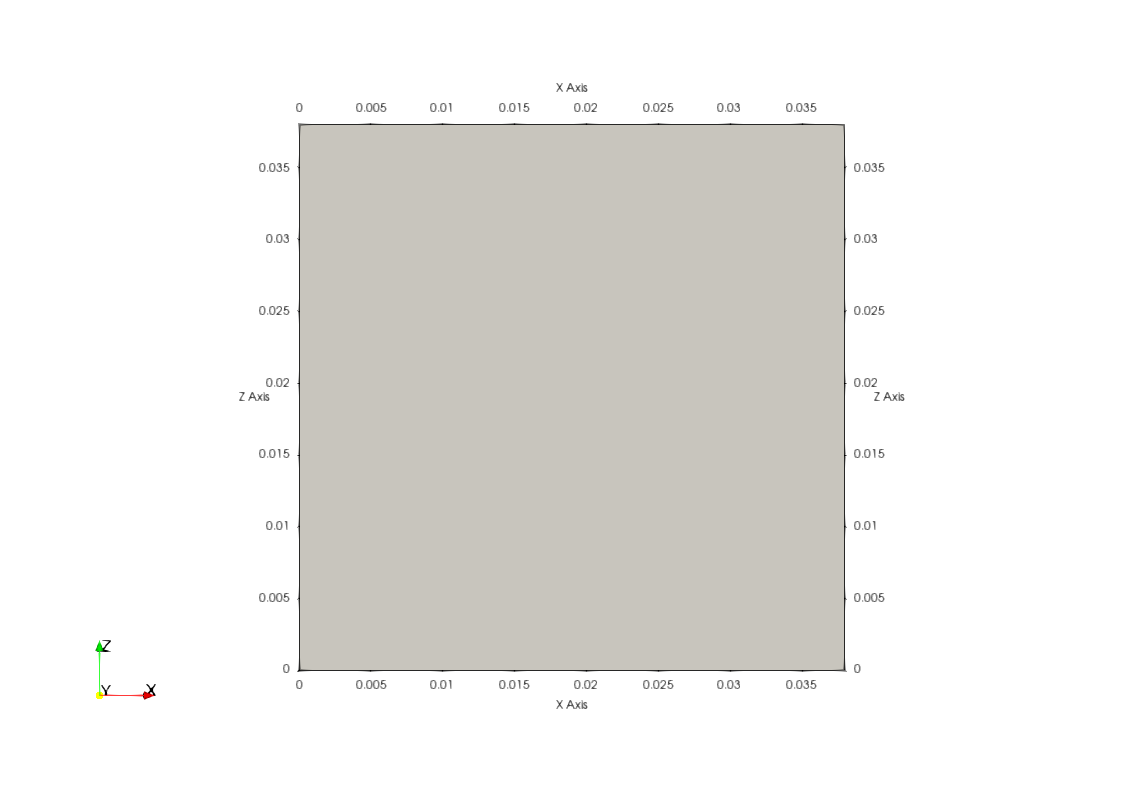
\includegraphics[width=.55\linewidth]{CF_GEOM.png}	
	\label{}
	\caption{Geometry of the case.}
\end{figure} 

\subsection{Hypotheses And Assumptions}

\subsection{Code implementations}
\subsection{Case Setup}
\subsubsection*{Boundary conditions}
\begin{table}[h!]
	\begin{tabular}{@{}lllll@{}}
		\toprule[1pt]
		\textbf{Boundary} & \textbf{Conditions}  \\ \midrule[2pt]
		Left & $T_{l}=283, v_{l} = 0   $  \\
		Right & $T_{r}=273, v_{r} = 0 $ \\
		Upper & $\frac{\partial T_{u}}{\partial n} = 0, v_{u} = 0$  \\
		Bottom & $\frac{\partial T_{b}}{\partial n} = 0, v_{b} = 0$  \\ \bottomrule[1pt]		
	\end{tabular}
	\centering
	\caption{Boundary conditions for natural convection case.}	
	\label{fig:boundaryCdsNaturalConvection}
\end{table}

\subsubsection*{Thermophysical properties}
\begin{table}[h!]
	\begin{tabular}{@{}lllll@{}}
		\toprule[1pt]
		\textbf{Water properties} & \textbf{Symbol} & \textbf{Values} & \textbf{Units} &  \\ \midrule[2pt]
		Density & $\rho_r$ & 999.8 & $kg.m^{-3}$ \\
		Dynamic viscosity & $\mu$ & 0.001003 & $kg.m^{-1}.s^{-1}$ \\
		Thermal conductivity & $\lambda$ & 0.6 & $W.m^{-1}.K^{-1}$ \\
		Heat capacity & $C_p$ & 4182 & $J.kg.K^{-1}$ \\		 
		Gravitational acceleration & $g$ &  9.81  & $m.s^{-2}$ \\
		Thermal diffusivity & $\gamma$ &  1.435e-7  & $m^{2}.s^{-1}$ \\		
		Thermal expansion coefficient & $\beta$ &  6.734e-5  & $K^{-1}$ \\	
		Laminar Prandtl number & $P_r$ &  6.99  & - \\
		Reference temperature & $T_r$ &  6.734e-5  & $K$ \\ \bottomrule[1pt]		
	\end{tabular}
	\centering
	\caption{Water properties for natural convection.}	
	\label{fig:waterProperties}
\end{table}

\subsubsection*{Solver parameters}
\begin{table}[h!]
	\begin{tabular}{@{}lllll@{}}
		\toprule[1pt]
		\textbf{Modeling Term} & \textbf{Keyword} & \textbf{Scheme} & \textbf{Remarks} &  \\ \midrule[2pt]
		Time derivatives & ddtSchemes    & Euler   &  \\
		Divergence term   &    &    &  \\
		Gradient term    & gradSchemes    &  Gauss linear  &  \\
		Laplacian term   &  laplacianSchemes    &  Gauss linear uncorrected   &  \\		 
		Others   		 & snGradSchemes    & uncorrected  &  \\ 
		&    			   interpolationSchemes    & linear  &  \\ \bottomrule[1pt]		
	\end{tabular}
		\centering
		\caption{Discretization schemes.}	
		\label{fig:boat3}
\end{table}
\begin{table}[h!]
	\begin{tabular}{@{}lllll@{}}
		\toprule[1pt]
		\textbf{Equation} & \textbf{Linear Solver} & \textbf{Smoother/Preconditioner} & \textbf{Tolerance} &  \\ \midrule[2pt]
		Pressure correction equation & PCG & DIC & 1e-8 \\
		Momentum equation & PBiCGStab & DILU  & 1e-6 \\
		Temperature equation & PBiCGStab & DILU  & 1e-6 \\\bottomrule[1pt]		
	\end{tabular}
	\centering
	\caption{Solvers for the discretised equations.}	
	\label{fig:boat4}
\end{table}
\begin{table}[h!]
	\begin{tabular}{@{}lllll@{}}
		\toprule[1pt]
		\textbf{Parameter} & \textbf{Value} & \textbf{Remarks} & \\ \midrule[2pt]
%		nAlphaCorr & PCG & DIC &  \\
%		nAlphaSubCycles & smoothSolver & symGaussSeidel  &  \\
%		cAlpha & smoothSolver & symGaussSeidel  &  \\
		momentumPredictor &  no    &    &  \\		 
		nOuterCorrectors &  1   &    &  \\ 
		nNonOrthogonalCorrectors &  0   &    &  \\ 		
		nCorrectors & 2	&    &  \\ \bottomrule[1pt]		
	\end{tabular}
	\centering
	\caption{Parameters for the discretised equations.}	
	\label{fig:boat5}
\end{table}

\subsection{Validation of Results and Conclusions}
\begin{figure}[h!]
	\begin{subfigure}{\linewidth}
	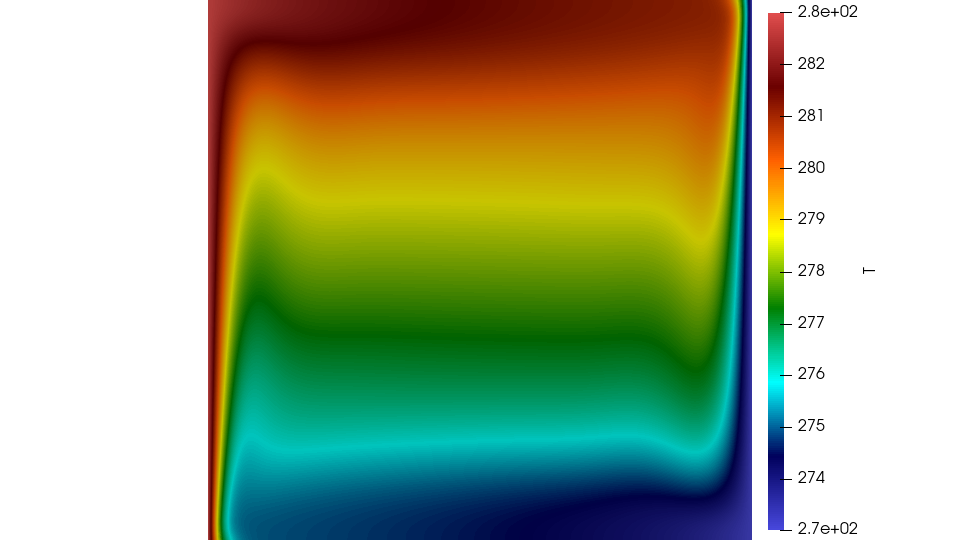
\includegraphics[width=.55\linewidth]{BBPF_T_1500s.png}\hfill
	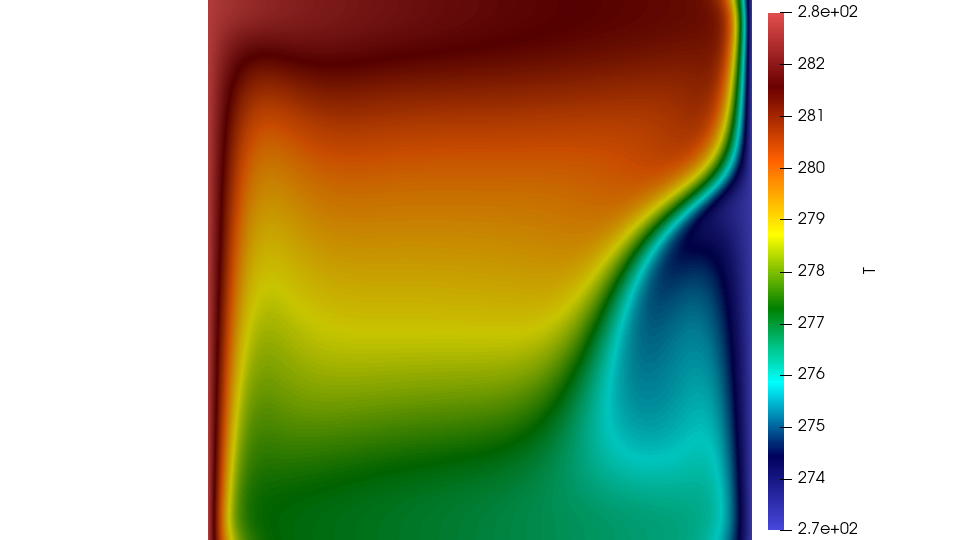
\includegraphics[width=.55\linewidth]{CF_T_1500s_comp.png}	
	\caption{Temperature magnitude comparison at t = 1500s. Left: BuoyantBoussinesqPimpleFoam. Right: NCMF}
	\label{BBPF_NCMF}
	\end{subfigure}\par\medskip
	\begin{subfigure}{\linewidth}
	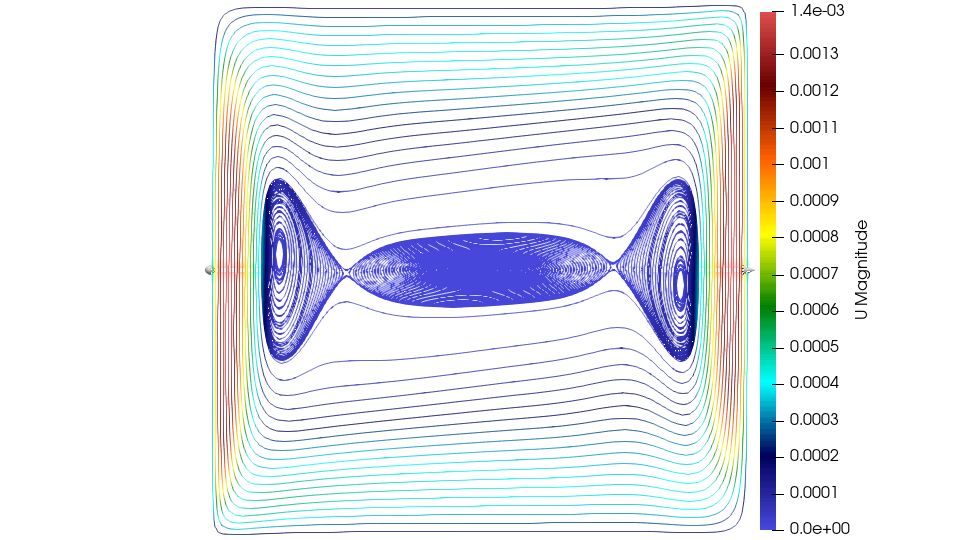
\includegraphics[width=.55\linewidth]{BBPF_U_1500s.png}\hfill
	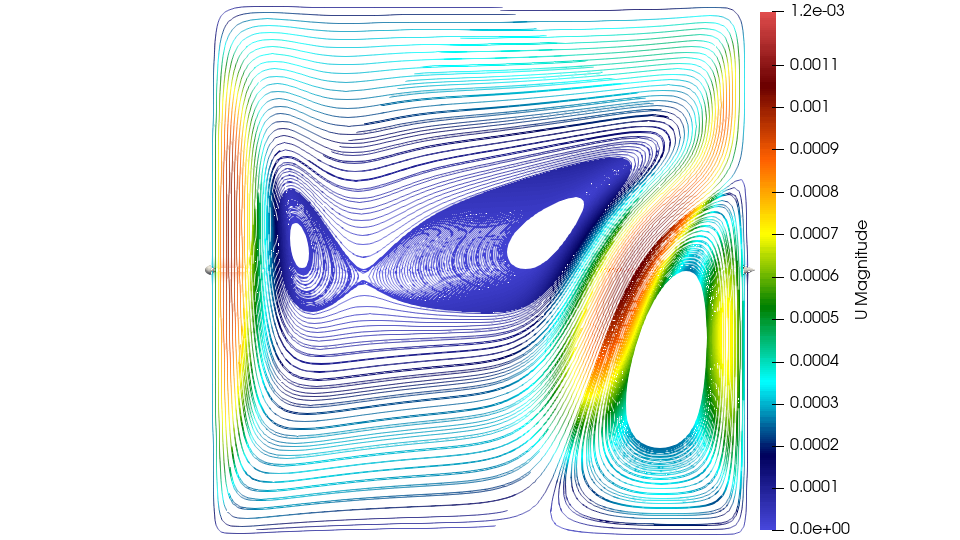
\includegraphics[width=.55\linewidth]{CF_U_1500s_comp.png}	
	\caption{Velocity magnitude comparison at t = 1500s. Left: BuoyantBoussinesqPimpleFoam. Right: NCMF}
	\end{subfigure}\par\medskip
	\caption{Comparison between BuoyantBoussinesqPimpleFoam and NCMF*}
\end{figure} 
NCMF*: Natural convection modified solver.
\begin{table}[h!]
	\begin{tabular}{@{}lllll@{}}
		\toprule[1pt]
		\multicolumn{1}{c}{\textbf{t = 100s}} & \multicolumn{1}{c}{\textbf{t = 250s}} & \multicolumn{1}{c}{\textbf{t = 1500s}} \\ \midrule[2pt] 
		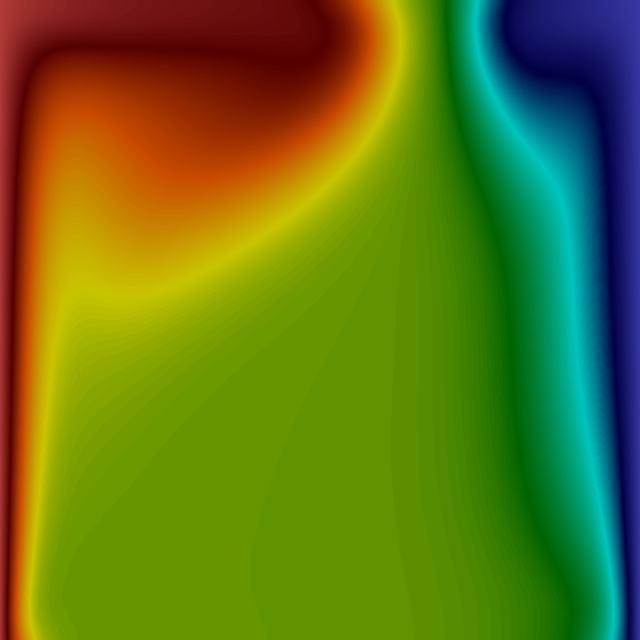
\includegraphics[width=.25\linewidth]{CF_T_100s.png} & 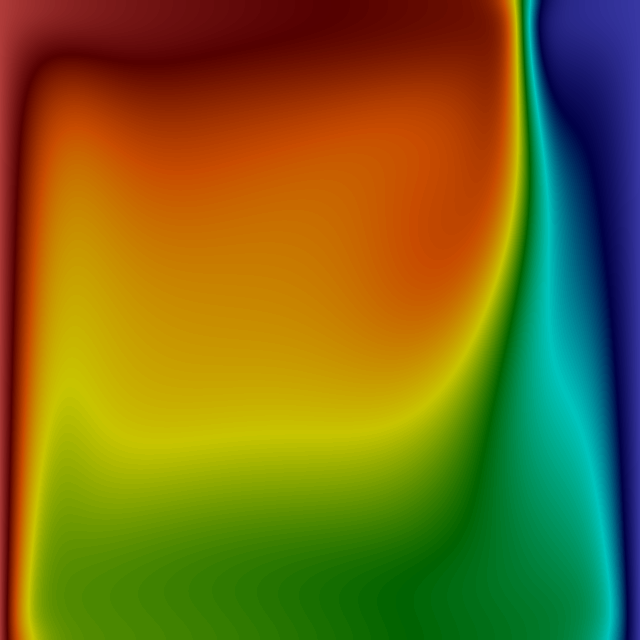
\includegraphics[width=.25\linewidth]{CF_T_250s.png} & 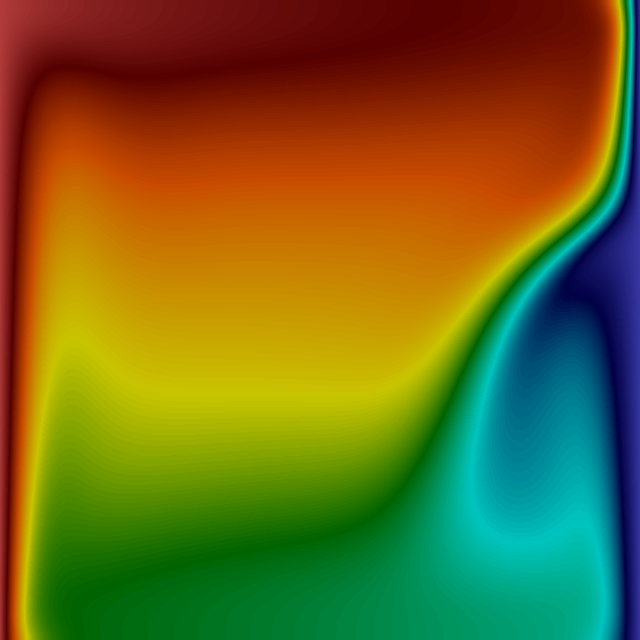
\includegraphics[width=.25\linewidth]{CF_T_1500s.png} & 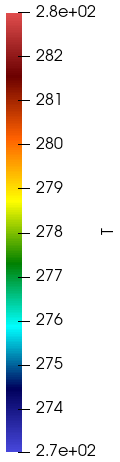
\includegraphics[width=.0658\linewidth]{t.png} \\
		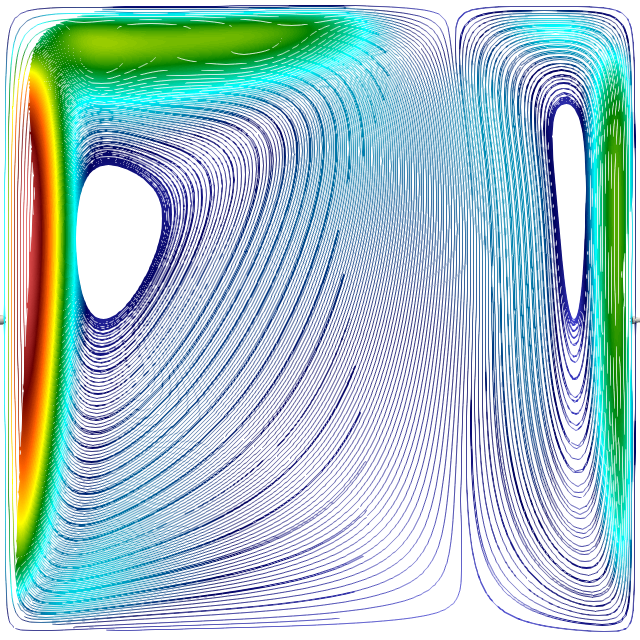
\includegraphics[width=.25\linewidth]{CF_U_100s.png} & 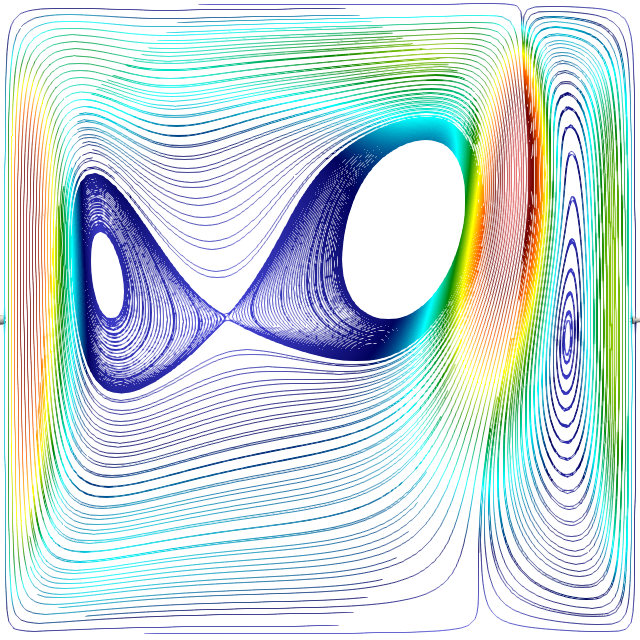
\includegraphics[width=.25\linewidth]{CF_U_250s.png} & 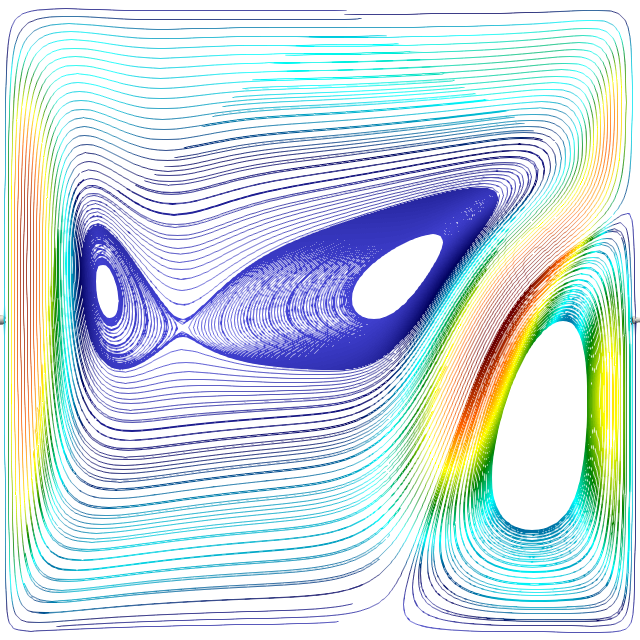
\includegraphics[width=.25\linewidth]{CF_U_1500s.png} & 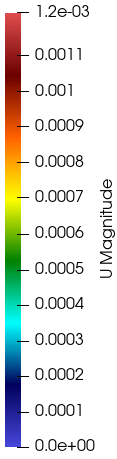
\includegraphics[width=.0658\linewidth]{u.png} \\
		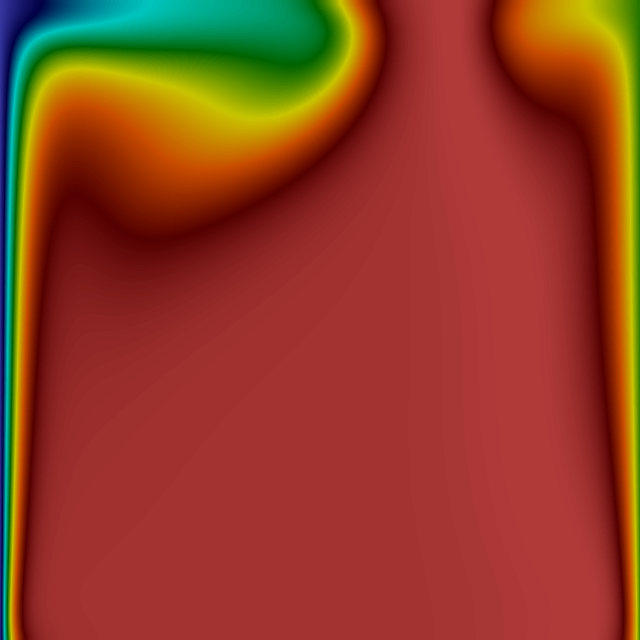
\includegraphics[width=.25\linewidth]{CF_rho_100s.png} & 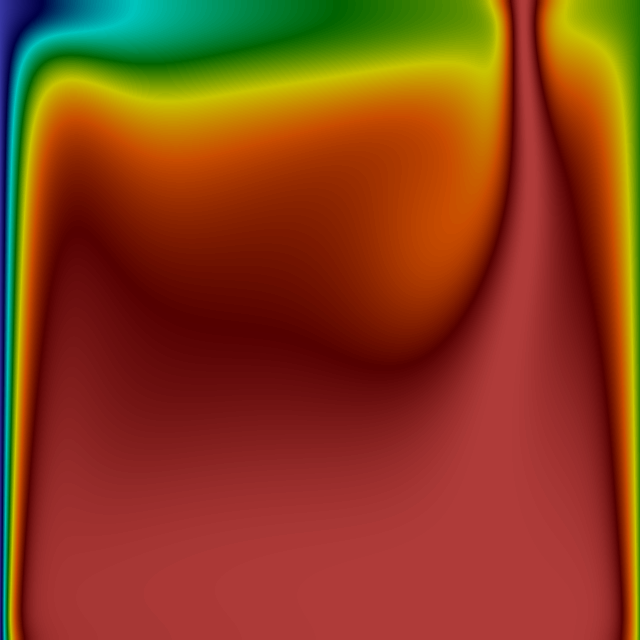
\includegraphics[width=.25\linewidth]{CF_rho_250s.png} & 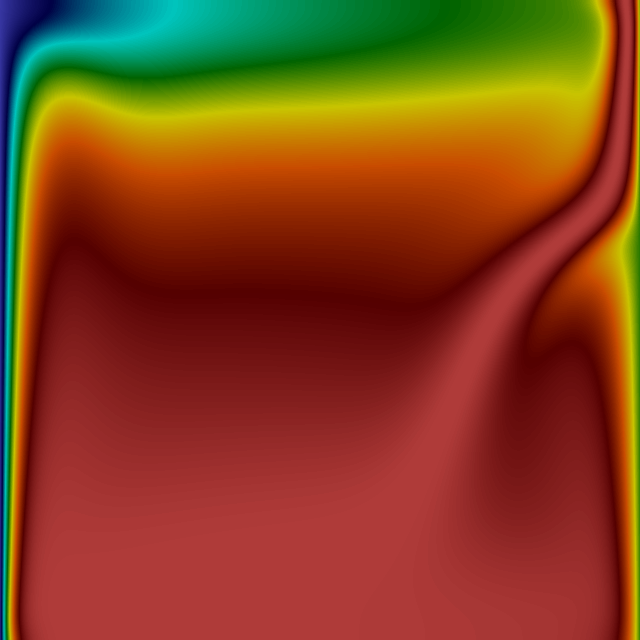
\includegraphics[width=.25\linewidth]{CF_rho_1500s.png} & 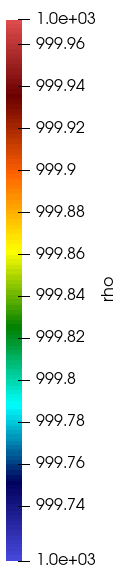
\includegraphics[width=.0558\linewidth]{rho.png} \\ \bottomrule[1pt]		
	\end{tabular}
	\centering
	\caption{Numerical results of Natural convection modified solver between \textit{t = 100s} and \textit{1500s}.}	
	\label{fig:resultsNCMF}
\end{table}
In order to compare consistently the obtained results with those of the literature, the following dimensionless values are pointed out:
\begin{equation}
	\tilde{T}=\frac{T-T_{\text {cold }}}{T_{\text {hot }}-T_{\text {cold }}}=\frac{T-273}{10}
	\label{}
\end{equation}
\begin{equation}
	\tilde{x}=\frac{x}{\ell}=\frac{x}{38 \times 10^{-3}}
	\label{}
\end{equation}
\begin{equation}
	\tilde{v}=\frac{v \ell}{\gamma}=\frac{v 38 \times 10^{-3}}{1.435 \times 10^{-7}}
	\label{}
\end{equation}
\begin{equation}
	\tilde{u}=\frac{u \ell}{\gamma}=\frac{u 38 \times 10^{-3}}{1.435 \times 10^{-7}}
	\label{}
\end{equation}
\begin{equation}
	\tilde{t}=\frac{t \gamma}{\ell^{2}}=\frac{t \times 1.435 \times 10^{-7}}{1.444 \times 10^{-6}}
	\label{}
\end{equation}
\begin{equation}
	\tilde{y}=\frac{y}{\ell}=\frac{y}{38 \times 10^{-3}}
	\label{}
\end{equation}
\newpage
\section{OpenFOAM: IcoReactingMultiphaseInterFOAM. Phase-Change Process}
IcoReactingMultiphaseInterFoam solver is a multiphase, multicomponent incompressible solver based on volume of fluid method. The solver captures the interfaces and includes contact angle and surface tension effects for each phase. Moreover, this solver supports mass and heat transfer across phases.
\newline
\subsection{Control Loop}

\subsection{Phase models}
The solver presents three phase model types:
\begin{itemize}
	\item \textbf{pureStaticSolidPhaseModel:} For pure static phase, like a solid.
	\item \textbf{pureMovingPhaseModel:} For pure moving phase, like a fluid.
	\item \textbf{multiComponentMovingPhaseModel:} For multi-component moving phase, like a multi-component fluid.
\end{itemize}
\subsection{Mass transfer models}
For each pair of phases, two mass transfer models might be used:
\begin{itemize}
	\item \textbf{Lee model:} Used for solid melting and liquid solidification.
	\item \textbf{KineticGasEvaporation:} Used for condensation and evaporation.
\end{itemize}
In this thesis, only the Lee model will be considered for further explanation.




\subsection{Governing Equations}
The solution of the system of equations given by the multiphase solver relies on a pressure-velocity coupling loop based on PISO (\textit{Pressure-Implicit with Splitting of Operators}). In order to give more stability to the solution and to simplify the boundary conditions, the pressure is treated by using a modified pressure:
\newline
Therefore, due to the commented before, the buoyancy terms appearing on the RHS of the momentum equation, are implemented on the pressure equation.

\subsubsection{Momentum Equation}

\subsubsection{Pressure Equation}

\subsubsection{Energy Equation}

\section{Case Description.}
For the solidification process, two geomtries are created: A squared and cylindrical plane geometries. 

\subsection{Hypotheses And Assumptions}
\subsection{Code implementations}
\subsection{Case Setup}
\subsubsection*{Boundary conditions}

For the squared cavity:
The initial conditions for the velocity and temperature fields are inherited from the last timestep of the natural convection case.
\begin{table}[h!]
	\begin{tabular}{@{}lllll@{}}
		\toprule[1pt]
		\textbf{Boundary} & \textbf{Conditions}  \\ \midrule[2pt]
		Left & $\frac{\partial \alpha_{l}}{\partial n} = 0, \frac{\partial \alpha_{s}}{\partial n} = 0    $  \\
		Right & $\alpha_{l} = inletOutlet* (1), \alpha_{l} = inletOutlet (0) $ \\
		Upper & $\frac{\partial \alpha_{l}}{\partial n} = 0, \frac{\partial \alpha_{s}}{\partial n} = 0$  \\
		Bottom & $\frac{\partial \alpha_{l}}{\partial n} = 0, \frac{\partial \alpha_{s}}{\partial n} = 0 $  \\ \bottomrule[1pt]		
	\end{tabular}
	\centering
	\caption{Boundary conditions for natural convection case.}	
	\label{fig:boundaryCdsCavity}
\end{table}
*inletOutlet is normally the same as zero gradient but it switches to fixed value if the velocity vector next to the boundary aims inside the domain.
For the cylinder:
\begin{table}[h!]
	\begin{tabular}{@{}lllll@{}}
		\toprule[1pt]
		\textbf{Boundary} & \textbf{Conditions}  \\ \midrule[2pt]
		Left & $T_{l}=283, v_{l} = 0   $  \\
		Right & $T_{r}=273, v_{r} = 0 $ \\
		Upper & $\frac{\partial T_{u}}{\partial n} = 0, v_{u} = 0$  \\
		Bottom & $\frac{\partial T_{b}}{\partial n} = 0, v_{b} = 0$  \\ \bottomrule[1pt]		
	\end{tabular}
	\centering
	\caption{Boundary conditions for natural convection case.}	
	\label{fig:boundaryCdsCylinder}
\end{table}
\subsubsection*{Thermophysical properties}
\begin{table}[h!]
	\begin{tabular}{@{}lllll@{}}
		\toprule[1pt]
		\textbf{Water properties} & \textbf{Symbol} & \textbf{Values} & \textbf{Units} &  \\ \midrule[2pt]
		Water density & $\rho_l$ & 999.8 & $kg.m^{-3}$ \\
		Ice density & $\rho_s$ & 916.8 & $kg.m^{-3}$ \\		
		Water kinematic viscosity & $\nu_{l}$ & 1.79e-6 & $m^{2}.s^{-1}$ \\
		Ice kinematic viscosity & $\nu_{s}$ & 2.0e-6 & $m^{2}.s^{-1}$ \\		
		Water thermal conductivity & $\lambda_{l}$ & 0.56 & $W.m^{-1}.K^{-1}$ \\
		Ice thermal conductivity & $\lambda_{s}$ & 2.26 & $W.m^{-1}.K^{-1}$ \\		
		Heat capacity & $C_{p_{l}}=C_{p_{s}}$ & 4202 & $J.kg.K^{-1}$ \\		 
		Gravitational acceleration & $g$ &  9.81  & $m.s^{-2}$ \\
		Thermal diffusivity & $\gamma$ &  1.435e-7  & $m^{2}.s^{-1}$ \\		
		Thermal expansion coefficient & $\beta$ &  6.734e-5  & $K^{-1}$ \\
		Latent heat & $L$ &  335000  & $J.K^{-1}$ \\			
		Laminar Prandtl number & $P_r$ &  6.99  & - \\
		Reference temperature & $T_r$ &  6.734e-5  & $K$ \\
		Darcy's constant & $D_c$ &  10e8  & - \\		 \bottomrule[1pt]		
	\end{tabular}
	\centering
	\caption{Water properties for natural convection.}	
	\label{fig:waterProperties}
\end{table}

Lee's model thermophysical parameters:

\subsubsection*{Two phase properties}
Within a multiphase framework, a model reflects a jump in properties through the interphase. Thus, a smooth transition between phase properties must be achieved.
\begin{equation}
\lambda=\lambda_{\ell} \alpha_{\ell}+\lambda_{s} f_{s}
\end{equation}
\begin{equation}
C_{p}=C_{p_{\ell}} \alpha_{\ell}+C_{p_{s}} f_{s}
\end{equation}
\begin{equation}
\mu=\mu_{\ell} \alpha_{\ell}+\mu_{s} f_{s}
\end{equation}

In the case of polynomial density variation it is settled in a similar manner. The polynomial is not thought to suit negative temperatures, and when the problem is within this range, the density should take ice's density.
\begin{equation}
\rho(T)^{\prime}=\rho(T) \alpha_{\ell}+\rho_{s} f_{s}
\end{equation}
\subsubsection*{Solver parameters}
\begin{table}[h!]
	\begin{tabular}{@{}lllll@{}}
		\toprule[1pt]
		\textbf{Modeling Term} & \textbf{Keyword} & \textbf{Scheme} & \textbf{Remarks} &  \\ \midrule[2pt]
		Time derivatives & ddtSchemes    &    &  \\
		Divergence term    &    &    &  \\
		Gradient term    & gradSchemes    &    &  \\
		Laplacian term   &  laplacianSchemes    &    &  \\		 
		Others   		 & snGradSchemes    &    &  \\ 
		&    			   interpolationSchemes    &    &  \\ \bottomrule[1pt]		
	\end{tabular}
	\centering
	\caption{Discretization schemes.}	
	\label{fig:boat3}
\end{table}
\begin{table}[h!]
	\begin{tabular}{@{}lllll@{}}
		\toprule[1pt]
		\textbf{Equation} & \textbf{Linear Solver} & \textbf{Smoother/Preconditioner} & \textbf{Tolerance} &  \\ \midrule[2pt]
		Pressure correction equation & PCG & DIC &  \\
		Momentum equation & smoothSolver & symGaussSeidel  &  \\
		Volume fraction equation & smoothSolver & symGaussSeidel  &  \\
		&      &    &  \\		 
		&     &    &  \\ 
		&    			       &    &  \\ \bottomrule[1pt]		
	\end{tabular}
	\centering
	\caption{Solvers for the discretised equations.}	
	\label{fig:boat4}
\end{table}
\begin{table}[h!]
	\begin{tabular}{@{}lllll@{}}
		\toprule[1pt]
		\textbf{Parameter} & \textbf{Value} & \textbf{Remarks} & \\ \midrule[2pt]
		nAlphaCorr & PCG & DIC &  \\
		nAlphaSubCycles & smoothSolver & symGaussSeidel  &  \\
		cAlpha & smoothSolver & symGaussSeidel  &  \\
		momentumPredictor &      &    &  \\		 
		nOuterCorrectors &     &    &  \\ 
		nNonOrthogonalCorrectors &     &    &  \\ 		
		nCorrectors &    			       &    &  \\ \bottomrule[1pt]		
	\end{tabular}
	\centering
	\caption{Parameters for the discretised equations.}	
	\label{fig:boat5}
\end{table}
\subsection{Validation of Results and Conclusions}
The validation of the phase change problem is achieved by different methodologies. First, the enthalpy-porosity method is compared with available data found in the thesis of \cite{bourdillon_2016} and \cite{kowalewski_rebow_1999}. For the Lee model based on the \textit{Classical Nucleation Theory}, the results are validated against the analytical solution given by the Neumann solutions of the Stefan problem.


\subsubsection{Stefan Problem}
The Stefan problem, is an initial boundary value problem of a parabolic differential equation with discontinuous coefficients on the phase transitions interfaces [\cite{vasilyev_vasilyeva_2020}]. The analytical solution to the classical Stefan problem exists in a limited range of idealized situations. Some of them involve semi-infinite or infinite regions with simple and boundary conditions. Based on the work of \cite{vasilyev_vasilyeva_2020} and \cite{zhao_zhao_xu_2018}, a two-region solidification process in a semi-infinite region is used to study the feasibility of the VOF-Lee model based on the Nucleation Theory.
\subsubsection*{One-dimensional problem}
In seek of simplification, and recalling the 1D problem as shown in the figure:

the initial conditions are expressed as:
\begin{equation}
	u_{0}(x)=u_{0}, \quad t=0, \quad x \in[0, L],
\end{equation}
while the boundary conditions are the shown below:
\begin{equation}
u(0, t)=-15ºC, \quad \frac{\partial u}{\partial x}(L, t)=0, \quad t>0
\end{equation}

The discontinuous exact solutions are:
\begin{equation}
	\begin{cases}T_{l}(x, t)=\frac{\operatorname{erfc}\left(\frac{x}{2 \sqrt{a_{1} t}}\right)}{\operatorname{erfc}\left(\lambda \sqrt{\frac{a_{\mathrm{s}}}{a_{1}}}\right)}\left(T_{\mathrm{m}}-T_{0}\right)+T_{0}, & x<\xi(t), \\ 
	T_{\mathrm{s}}(\chi, t)=\frac{\operatorname{erf}\left(\frac{x}{2 \sqrt{a_{\mathrm{s}} t}}\right)}{\operatorname{erf \cdot\lambda }}\left(T_{\mathrm{m}}-T_{\mathrm{b}}\right)+T_{\mathrm{b}},& x \geq \xi(t)  .\end{cases}
\end{equation}
By using a phase change interface condition, a solution to the trascendental equation may be found:
\begin{equation}
	\frac{e^{-\lambda^{2}}}{\operatorname{erf}(\lambda)}+\frac{k_{\mathrm{l}}}{k_{\mathrm{s}}} \sqrt{\frac{a_{\mathrm{s}}}{a_{1}}} \frac{T_{\mathrm{m}}-T_{0}}{T_{\mathrm{m}}-T_{\mathrm{b}}} \frac{e^{-\frac{a_{\mathrm{s}}}{a_{1}} \lambda^{2}}}{\operatorname{erfc}\left(\lambda \sqrt{\frac{a_{\mathrm{s}}}{a_{1}}}\right)}=\frac{\lambda L \sqrt{\pi}}{c_{\mathrm{ps}}\left(T_{\mathrm{m}}-T_{\mathrm{b}}\right)}
\end{equation}
The secant method is used as the iterative scheme to find the root of the given function with $tol<1e-12$. The root of $\gamma$ is 0.2204835149063661

The evolution of the interface is:
\begin{equation}
	X(t)=2 \lambda \sqrt{a_{\mathrm{s}} t}
\end{equation}
%The discontinuous exact solution is of the form [\cite{vasilyev_vasilyeva_2020}:
%\begin{equation}
%	u(x, t)= \begin{cases}g\left[\operatorname{erf}\left(\frac{\xi}{2 a_{1} \sqrt{t}}\right)-\operatorname{erf}\left(\frac{x}{2 a_{1} \sqrt{t}}\right)\right] / \operatorname{erf}\left(\frac{\xi}{2 a_{1} \sqrt{t}}\right), & x \geq \xi(t), \\ u_{0}\left[\operatorname{erf}\left(\frac{x}{2 a_{2} \sqrt{t}}\right)-\operatorname{erf}\left(\frac{\xi}{2 a_{2} \sqrt{t}}\right)\right] /\left[1-\operatorname{erf}\left(\frac{\xi}{2 a_{2} \sqrt{t}}\right)\right], & x<\xi(t) .\end{cases}
%\end{equation}
%
%By using a phase change interface condition, it is possible to find a solution to the trascendental equation.
%\begin{equation}
%	\frac{k_{1}}{a_{1}} g \frac{\exp \left(-\left(\frac{\gamma}{2 a_{1}}\right)^{2}\right)}{\operatorname{erf}\left(\frac{\gamma}{2 a_{1}}\right)}+\frac{k_{2}}{a_{2}} u_{0} \frac{\exp \left(-\left(\frac{\gamma}{2 a_{2}}\right)^{2}\right)}{1-\operatorname{erf}\left(\frac{\gamma}{2 a_{2}}\right)}+\gamma D \frac{\sqrt{\pi}}{2}=0
%\end{equation}
%
%The secant method is used as the iterative scheme to find the root of the given function with $tol<1e-12$. The root of $\gamma$ is 0.00032622525325939834
